Artificial intelligence is a pretty useful tool, as long as it doesn't
get too smart. Of course, that's the situation you find yourself in now,
as your Piloting ALgorithm (PAL) has refused to direct your ship 
into a particularly dangerous system.

PAL concedes that it will let you proceed, but only if can complete
extract the secret word hidden within its \textbf{Cubic Monolith}.
To do so, you'll need to adhere to the illustrated rules for
placing the numbers \(1\) through \(4\) in rows, columns, towers, and cages.

%\begin{itemize}
%\item Each row of a level must contain exactly one
%  of the numbers 1,2,3,4.
%\item Each column of a level must contain exactly one
%  of the numbers 1,2,3,4.
%\item Each tower of the cube must contain exactly one
%  of the numbers 1,2,3,4.
%\item All the numbers within each solid-boundary cage
%  (possibly connected by arrows to other levels) of the cube 
%  either add or multiply to 12.
%\end{itemize}

\begin{center}
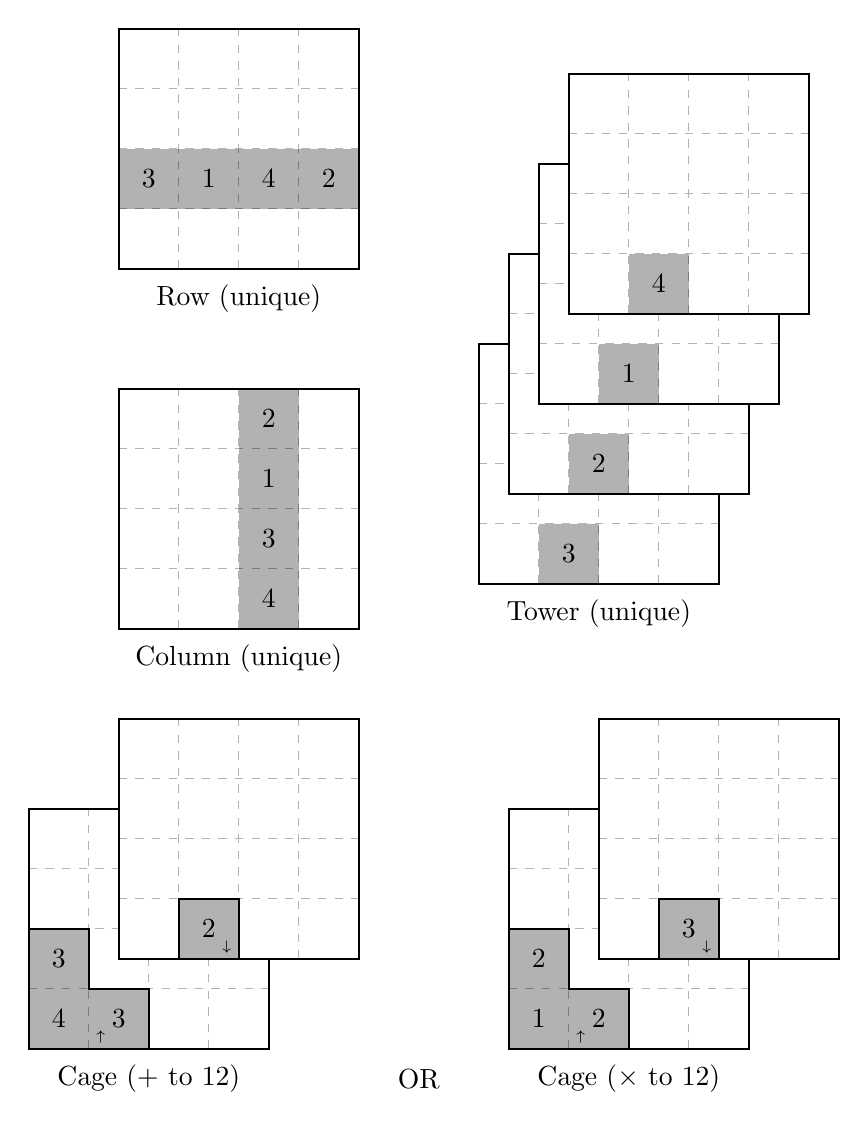
\begin{tikzpicture}[x=0.3in,y=0.3in]
\begin{scope}[shift={(-0.5,0)}]
\draw[fill=white] (0,0) rectangle (4,4);
\draw[step=1,dashed,color=black!30] (0,0) grid (4,4);
\draw[thick] (0,0) rectangle (4,4);
\fill[opacity=0.3] (0,1) rectangle (4,2);
\node at (2,-0.5) {Row (unique)};
\node at (0.5,1.5) {3};
\node at (1.5,1.5) {1};
\node at (2.5,1.5) {4};
\node at (3.5,1.5) {2};
\end{scope}
\begin{scope}[shift={(-0.5,-6)}]
\draw[fill=white] (0,0) rectangle (4,4);
\draw[step=1,dashed,color=black!30] (0,0) grid (4,4);
\draw[thick] (0,0) rectangle (4,4);
\fill[opacity=0.3] (2,0) rectangle (3,4);
\node at (2,-0.5) {Column (unique)};
\node at (2.5,0.5) {4};
\node at (2.5,1.5) {3};
\node at (2.5,2.5) {1};
\node at (2.5,3.5) {2};
\end{scope}
\begin{scope}[shift={(5.5,-5.25)}]
\draw[fill=white] (0,0) rectangle (4,4);
\draw[step=1,dashed,color=black!30] (0,0) grid (4,4);
\draw[thick] (0,0) rectangle (4,4);
\fill[opacity=0.3] (1,0) rectangle (2,1);
\node at (2,-0.5) {Tower (unique)};
\node at (1.5,0.5) {3};
  \begin{scope}[shift={(0.5,1.5)}]
  \draw[fill=white] (0,0) rectangle (4,4);
  \draw[step=1,dashed,color=black!30] (0,0) grid (4,4);
  \draw[thick] (0,0) rectangle (4,4);
  \fill[opacity=0.3] (1,0) rectangle (2,1);
  \node at (1.5,0.5) {2};
  \begin{scope}[shift={(0.5,1.5)}]
  \draw[fill=white] (0,0) rectangle (4,4);
  \draw[step=1,dashed,color=black!30] (0,0) grid (4,4);
  \draw[thick] (0,0) rectangle (4,4);
  \fill[opacity=0.3] (1,0) rectangle (2,1);
  \node at (1.5,0.5) {1};
  \begin{scope}[shift={(0.5,1.5)}]
  \draw[fill=white] (0,0) rectangle (4,4);
  \draw[step=1,dashed,color=black!30] (0,0) grid (4,4);
  \draw[thick] (0,0) rectangle (4,4);
  \fill[opacity=0.3] (1,0) rectangle (2,1);
  \node at (1.5,0.5) {4};
  \end{scope}
  \end{scope}
  \end{scope}
\end{scope}
\begin{scope}[shift={(-2,-13)}]
\draw[fill=white] (0,0) rectangle (4,4);
\draw[step=1,dashed,color=black!30] (0,0) grid (4,4);
\draw[thick] (0,0) rectangle (4,4);
\fill[opacity=0.3] (0,2) -- (1,2) -- (1,1) -- (2,1) -- (2,0) -- (0,0) -- (0,2);
\draw[thick] (0,2) -- (1,2) -- (1,1) -- (2,1) -- (2,0);
\node at (2,-0.5) {Cage (\(+\) to \(12\))};
\node at (1.5,0.5) {3};
\node at (0.5,0.5) {4};
\node at (0.5,1.5) {3};
\node at (1.2,0.2) {\tiny\(\uparrow\)};
  \begin{scope}[shift={(1.5,1.5)}]
  \draw[fill=white] (0,0) rectangle (4,4);
  \draw[step=1,dashed,color=black!30] (0,0) grid (4,4);
  \draw[thick] (0,0) rectangle (4,4);
  \draw[thick] (1,0) rectangle (2,1);
  \fill[opacity=0.3] (1,0) rectangle (2,1);
  \node at (1.5,0.5) {2};
  \node at (1.8,0.2) {\tiny\(\downarrow\)};
  \end{scope}
\end{scope}
\node at (4.5,-13.5) {OR};
\begin{scope}[shift={(6,-13)}]
\draw[fill=white] (0,0) rectangle (4,4);
\draw[step=1,dashed,color=black!30] (0,0) grid (4,4);
\draw[thick] (0,0) rectangle (4,4);
\fill[opacity=0.3] (0,2) -- (1,2) -- (1,1) -- (2,1) -- (2,0) -- (0,0) -- (0,2);
\draw[thick] (0,2) -- (1,2) -- (1,1) -- (2,1) -- (2,0);
\node at (2,-0.5) {Cage (\(\times\) to \(12\))};
\node at (1.5,0.5) {2};
\node at (0.5,0.5) {1};
\node at (0.5,1.5) {2};
\node at (1.2,0.2) {\tiny\(\uparrow\)};
  \begin{scope}[shift={(1.5,1.5)}]
  \draw[fill=white] (0,0) rectangle (4,4);
  \draw[step=1,dashed,color=black!30] (0,0) grid (4,4);
  \draw[thick] (0,0) rectangle (4,4);
  \draw[thick] (1,0) rectangle (2,1);
  \fill[opacity=0.3] (1,0) rectangle (2,1);
  \node at (1.5,0.5) {3};
  \node at (1.8,0.2) {\tiny\(\downarrow\)};
  \end{scope}
\end{scope}
\end{tikzpicture}
\end{center}
